\chapter{Architecture}

\section{System Context}
We have a single \emph{JassTracker} system without any external services.

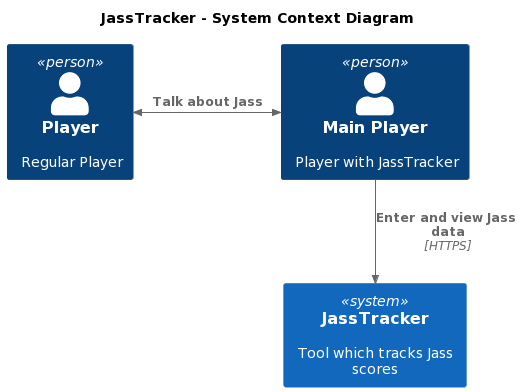
\includegraphics[width=0.6\textwidth]{resources/diagrams/c4-1-system-context}

\section{Container}
Our system is split into three containers.
Each container uses its own technology and could be (relatively) easily exchanged.

The \emph{Frontend} is our single-page-application which provides the user interface.
We decided to use a dedicated SPA instead of server rendered pages to improve the user experience.
When a user enters a score, only a small fraction of the whole page needs to be updated.
We can also stay more flexible with a dedicated SPA, and for example, we could implement an offline mode in the future.

The \emph{Backend} provides multiple REST-API-Endpoints, which will be used by the \emph{Frontend}.
All business logic will be implemented and tested here, providing preprocessed and easy to digest data upon request.
Having a public REST-API enforces a clean separation and makes testing early on easier.

The \emph{Database} is a simple PostgreSQL database used to store our data.
It is part of the JassTracker system, and therefore it gets set up, deployed and migrated in conjunction with the other components.
This approach lets us effortlessly manage multiple instances of the same system without manually having to keep databases up to date.

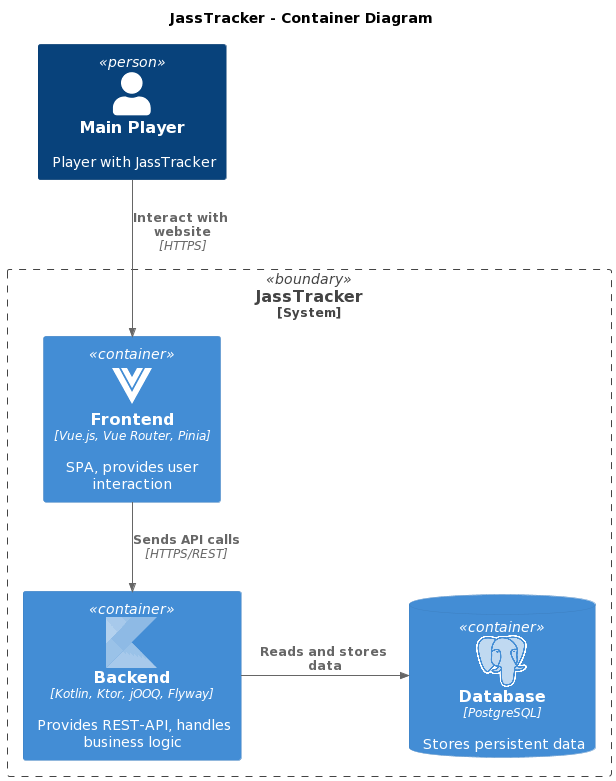
\includegraphics[width=0.6\textwidth]{resources/diagrams/c4-2-container}

\section{Components}

\subsection{Frontend}
The frontend is a single-page-application written in Vue3 and TypeScript.
We use Vue \emph{Single-File Components}, keeping all relevant parts of a component in a single file.
TypeScript ensures more issues are caught at compile time, reducing testing overhead.

\subsubsection*{Store}
We use \href{https://pinia.vuejs.org/}{Pinia} as a state store, which is the modern default for Vue3.
Using a central state was a deliberate decision to ensure a clean separation of concerns.
We can have most business logic in a central, testable and re-usable place.
Pinia also provides a great developer experience for understanding the current state of the application.

\subsubsection*{Views}
Every route (e.g. \emph{/overview}, \emph{/profile}) is implemented as a view.
These views are responsible for tying together different components and the state store.
Relevant data is requested from the store and provided to components.

\subsubsection*{Components}
Whenever any piece of UI code wants to be re-used, it's put in a component.
These components get used across many views without knowing in which it gets used.
A component has simple input and output using Vue mechanics that make them flexible.
This separation ensures re-usability without requiring refactoring first.

\subsubsection*{Services}
Services provide a small abstraction layer to the backend.
The services are strictly typed, which enables frontend developers to write code without having to look at the backend api definition.
The \href{https://github.com/posva/mande}{mande} dependency is very simple, which facilitates the creation of services.

\subsection{Backend}
The backend is structured into circular layers, following the clean-architecture principle.
This means that the \emph{Domain} is in the center, being responsible for all business logic.
Technology-dependent logic is extracted to an outer layer, ensuring they could be easily changed in the future.

\subsubsection*{Bootstrap}
The bootstrap module was created as an entry point to the backend.
It reads the configuration file, configures the web server and initializes all modules.
This module is the least testable and depends on everything else, that's why as little logic as possible is stored here.
Still, one key part of the Bootstrap module is configuring Ktor, we decided that a dedicated module for Ktor configuration would provide little benefit.

\subsubsection*{Security}
The security module is our smallest module, but it's still essential.
Password hashing and JWT configuration get done within this module to abstract any security related dependencies.
If anything cryptography-related wasn't correct, this would be the place to fix it.

\subsubsection*{Web API}
The web API module provides the JassTracker services over a REST API\@.
All framework specific code for handling a request, like loading URL parameters or reading headers, is done here.

\subsubsection*{Data Access}
The data access module is an abstraction layer to the database.
It also encapsulates data migration and other database-specific tasks.
No other module knows the specific database, not even if it's a database at all.
This gives us great flexibility and testability, for example for using an in-memory database if we so desire.
All public services implemented by this module are called \emph{Repository} by convention.

\subsubsection*{Domain}
The domain module contains the technology independent business logic.
It handles whose turn it is, calculates advanced statistics, performs extended input validation etc.
If you wanted to create a fat desktop client for the JassTracker, you would be able to re-use this domain module.

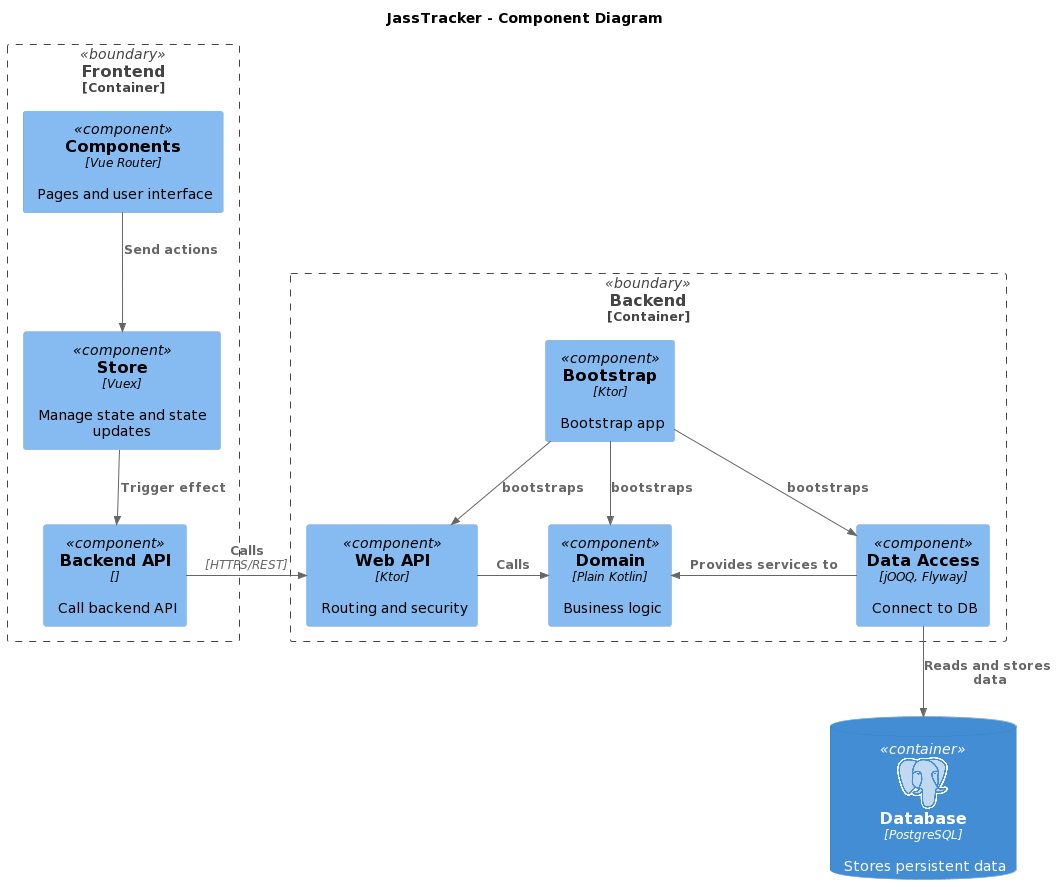
\includegraphics[width=0.9\textwidth]{resources/diagrams/c4-3-component}

\section{Tools \& Frameworks}

In general, our technologies were chosen with simplicity and maintainability in mind.
We wanted a tech-stack which was relatively easy to learn, while still allowing for clean and extensible architecture.
This overview does not aim to provide details into each technology, but a one-sentence summary on why it was chosen.

\subsection*{Frontend}

\begin{compactitem}
    \item \textbf{vue} is a simple frontend framework which meets our requirements
    \item \textbf{mande} is a basic wrapper around fetch, which reduces boilerplate
    \item \textbf{pinia} is the new standard state management solution from Vue.js
    \item \textbf{vue-draggable-next} implements the drag-and-drop functionality we needed
    \item \textbf{vue-toastification} has beautiful toast messages with a Vue.js 3 compatible API
    \item \textbf{vue3-charts} provides a very simple Vue.js 3 API for all the charts we need
    \item \textbf{eslint} is the state-of-the-art linter for TypeScript and JavaScript
    \item \textbf{sass} is a powerful css preprocessor which allows us to re-use styles effectively
    \item \textbf{prettier} is an opinionated formatter which integrates with ESlint and IntelliJ
    \item \textbf{tailwindcss} provides a modern way of designing web-apps by applying utility classes instead of writing custom CSS rules
    \item \textbf{typescript} allows for strict typing to detect a number of errors at compile-time
\end{compactitem}

\subsection*{Backend}

\begin{compactitem}
    \item \textbf{Kotlin} is a modern programming language with many productivity benefits over Java
    \item \textbf{Ktor} is a simple and fun server framework, which is easy to understand and work with
    \item \textbf{Kotlinx-Serialization} is the official serialization solution from Kotlin and provides great performance
    \item \textbf{Kotlinx-Datetime} provides a plattform-independent API similar to java.time
    \item \textbf{Argon2} won the Password Hashing Competition (PHC) and is used to hash player passwords
    \item \textbf{jOOQ} is a SQL wrapper for the JVM, which is simple to use if you already know SQL
    \item \textbf{Java-JWT} is used by Ktor when using JWT tokens, which are an industry standard for representing security claims
    \item \textbf{Flyway} is a database migration tool with a simple setup and SQL-based migrations
    \item \textbf{shadow} is used to build a fat JAR for use within docker containers
    \item \textbf{Kotlin-Test} provides test annotations and utilities with great Kotlin integration
    \item \textbf{Ktor-Server-Tests} is the testing counterpart to Ktor, allowing us to write
    \item \textbf{Mockk} is the most popular Kotlin mocking framework
    \item \textbf{Testcontainers} allow us to run integrations tests against a real Postgres database
\end{compactitem}

\section{Code}
It is best to illustrate how these components work together by an example.
When a user logs in, he will arrive at an endpoint specified within the web API module.
The web API then proceeds to parse the payload and map it to a call into the domain module.
If the endpoint is authenticated, the current user will be read from the provided JWT header and passed along.

Once in the domain module, business logic happens, other services are called etc.
For example, for a login, you'll have to load the player by username from the repository.
The domain doesn't know or care about the exact way a player is found, but it expects a domain player to be returned.
Therefore, the repository implementation within the data-access module has to map the database records to the correct domain object.

Once the domain code has decided that the login is valid, a JWT token is created by calling an AuthTokenService.
This service resides within the security module, but the domain doesn't know that.
Thanks to Dependency Injection, the business logic stays completely isolated from technical dependencies.

The token created by the domain is finally returned to the web API, which will ensure the token is returned in a valid JSON to the caller.
If the login had failed, the domain would've returned null instead of a valid token.
In that case, the web API can decide on how to handle an invalid login, for example by returning an HTTP 400 response.

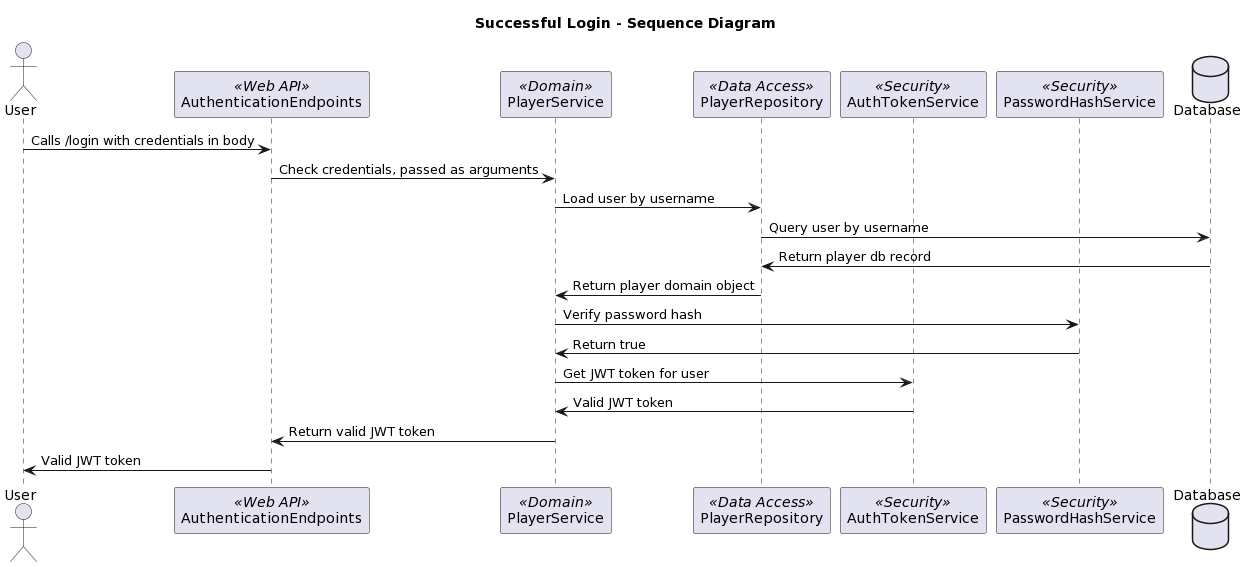
\includegraphics[width=\textwidth]{resources/diagrams/login-sequence}

\newpage

\section{Deployment Overview}
\label{sec:architecture_deployment}
Our deployment architecture strives for maximum simplicity while remaining flexible and extensible.
To achieve that goal, a few decisions were made:
\begin{itemize}
    \item use a single host to keep it simple
    \item use docker to make deployments portable
    \item use a reverse proxy to enable a separate \href{https://jasstracker-test.honegger.dev}{staging} and \href{https://jasstracker.honegger.dev}{prod} environments
    \item use one database container for all environments to preserve resources
\end{itemize}

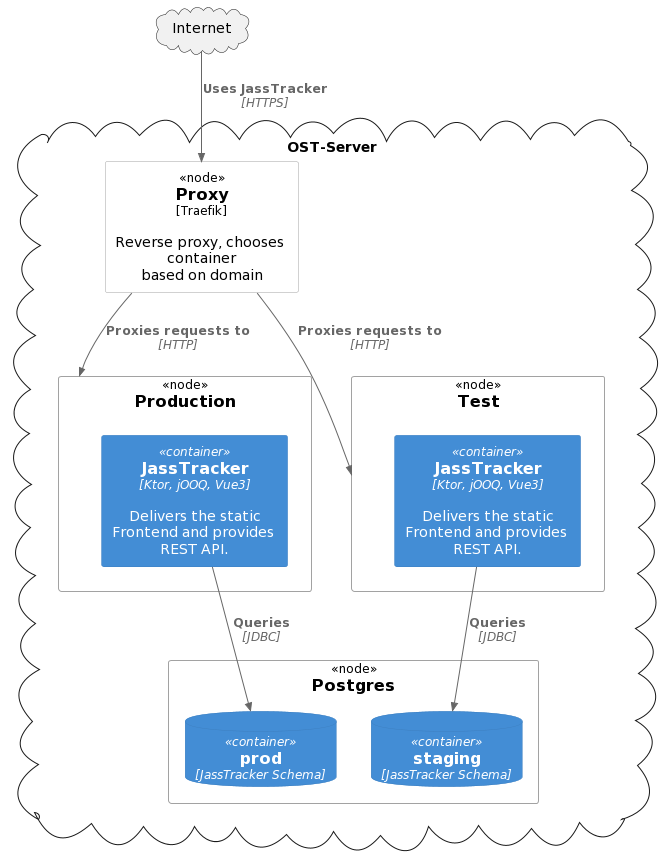
\includegraphics[width=0.8\textwidth]{resources/diagrams/c4-deployment}
